\documentclass{beamer}

\usepackage{centernot}
\usetheme{Boadilla}
% \usepackage{beamerthemesplit} // Activate for custom appearance

\title{Time, Clocks, and the Ordering of Events in a Distributed System}
\subtitle{Leslie Lamport}
\author{Yuncong Zhang}
\date{April 23, 2020}

\begin{document}

\frame{\titlepage}

\frame{\frametitle{Outline}\tableofcontents}

\section{Total Ordering of Events}

\frame
{
  \frametitle{Events in Distributed System}
	\begin{columns}
	\begin{column}{0.6\textwidth}

		\onslide<+-> What does it mean by ``$a$ happens before $b$'' in distributed system?

		\begin{itemize}
			\item<+-> Hard to define across asynchornized processes
			\item<+-> In one process, \textbf{earlier} events happens before \textbf{later} events
			\item<+-> \textbf{Sending message} happens before \textbf{receiving message}
			\item<+-> If $a$ happens before $b$, and $b$ happens before $c$, then $a$ happens before $c$
		\end{itemize}

	\end{column}
	\begin{column}{0.4\textwidth}

		\begin{figure}[ht!]
		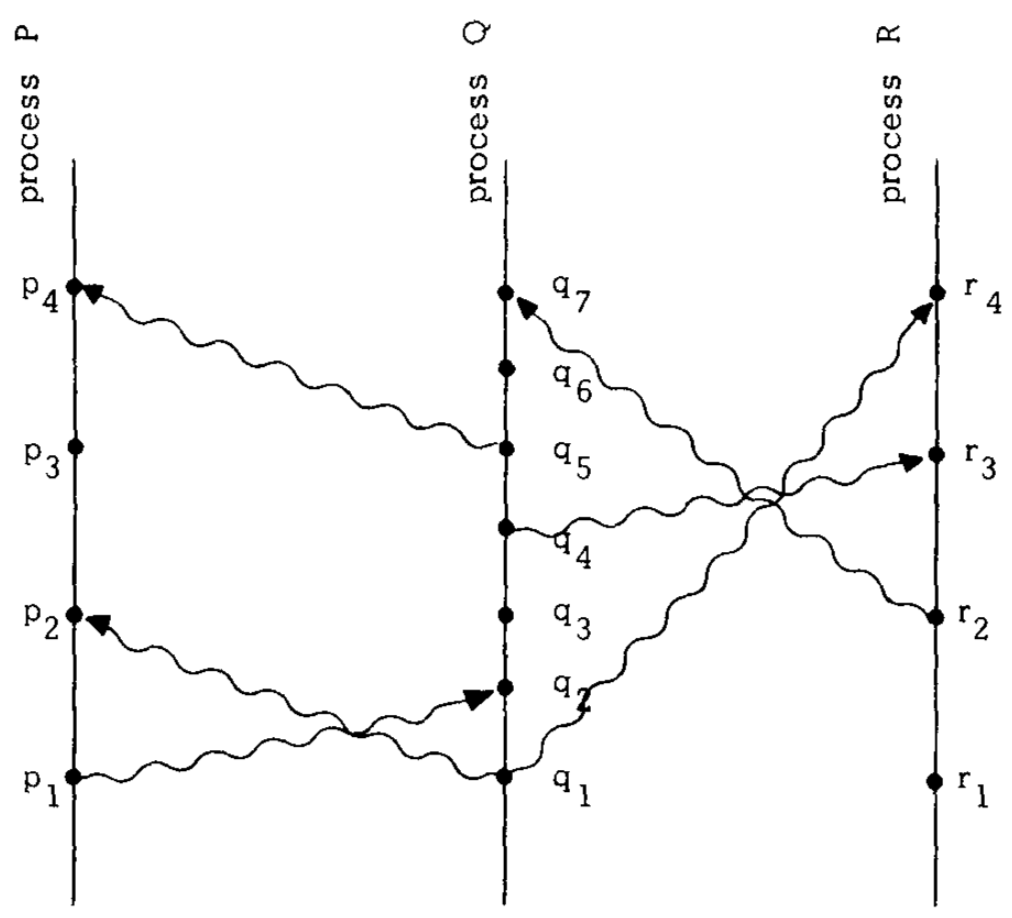
\includegraphics[width=\textwidth]{files/events-messages.png}
		\end{figure}


	\end{column}
	\end{columns}
}

\frame
{
  \frametitle{Partial Ordering of Events}
	\begin{columns}
	\begin{column}{0.6\textwidth}

		Denote by $a\to b$ if $a$ happens before $b$.

		\begin{itemize}
			\item<2-> ``$\to$'' defines a partial order: not all pairs of events are ordered
			\item<3-> If $a\nrightarrow b$ and $b\nrightarrow a$ then $a$ and $b$ are \emph{concurrent}
			\item<4-> $a\to b$ is equivalent to saying one can go from $a$ to $b$ in the diagram by moving forward in time along process and message lines.
		\end{itemize}


	\end{column}
	\begin{column}{0.4\textwidth}

		\begin{figure}[ht!]
		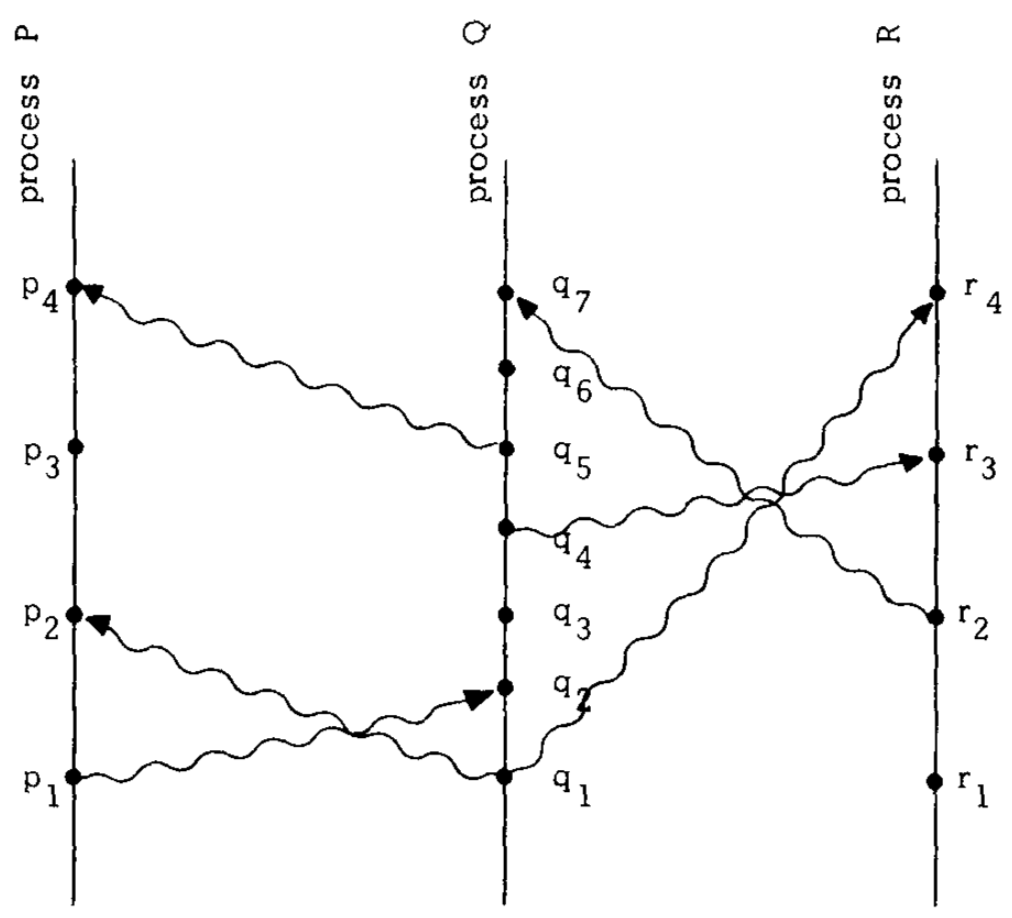
\includegraphics[width=\textwidth]{files/events-messages.png}
		\end{figure}


	\end{column}
	\end{columns}

}

\frame
{
  \frametitle{Partial Ordering of Events}
	\begin{columns}
	\begin{column}{0.6\textwidth}

		Example: $p_1\to r_4$
		\begin{itemize}
			\item<2-> $p_1\to q_2$
			\item<3-> $q_2\to q_4$
			\item<4-> $q_4\to r_3$
			\item<5-> $r_3\to r_4$
		\end{itemize}


	\end{column}
	\begin{column}{0.4\textwidth}

		\begin{figure}[ht!]
		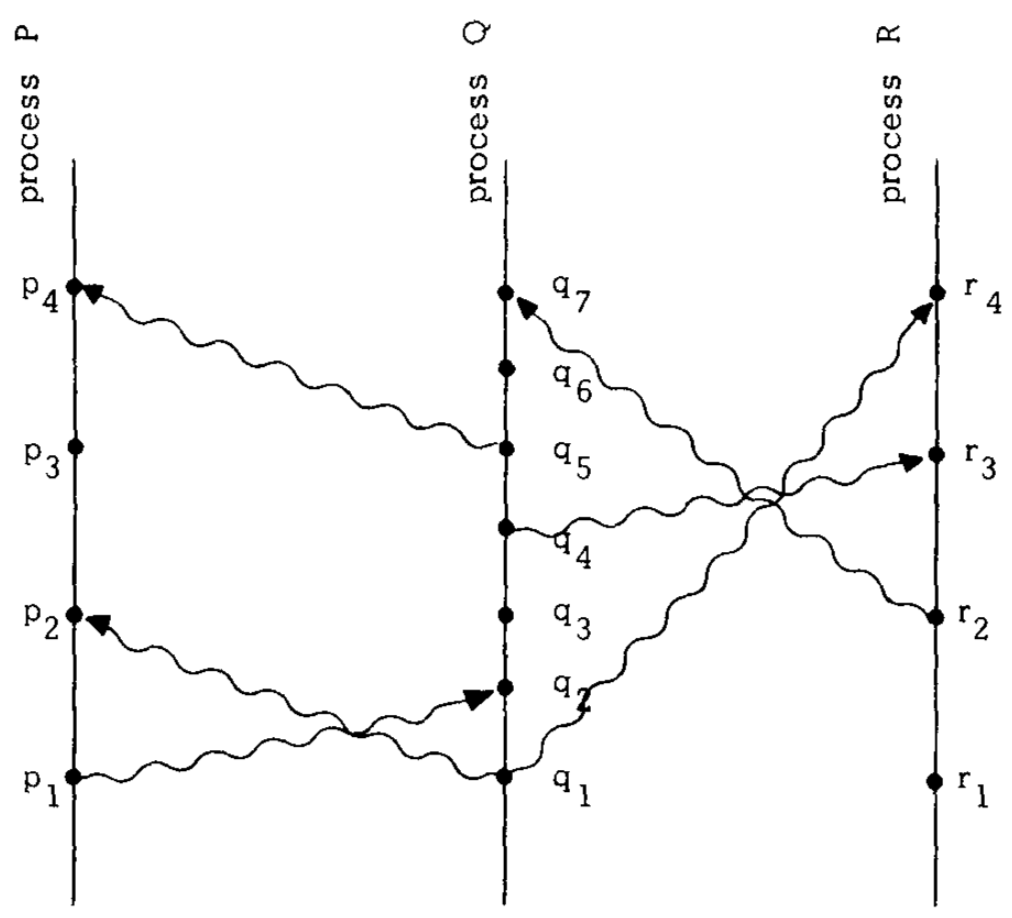
\includegraphics[width=\textwidth]{files/events-messages.png}
		\end{figure}


	\end{column}
	\end{columns}

}

\frame
{
	\frametitle{Logical Clocks}

	\begin{columns}
	\begin{column}{0.6\textwidth}

		Logical clock is an assignment of numbers on events
		\begin{itemize}
			\item<2-> Local clock $C_i$ assigns number $C_i\langle a\rangle$ to event $a$ in process $P_i$
			\item<3-> Global clock $C$ defined by $C\langle a\rangle=C_i\langle a\rangle$ if $a$ is in process $P_i$
		\end{itemize}


	\end{column}
	\begin{column}{0.4\textwidth}

		\begin{figure}[ht!]
		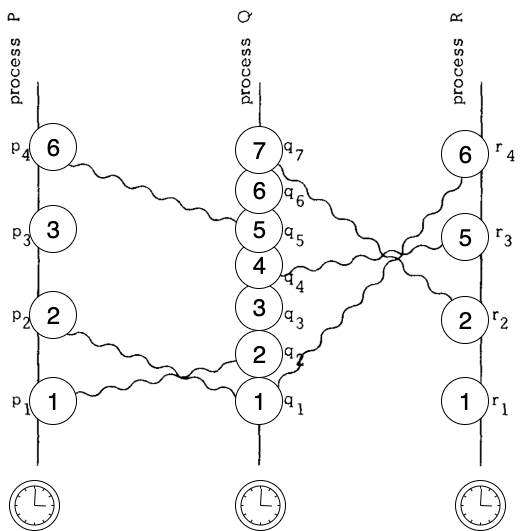
\includegraphics[width=\textwidth]{files/ClockDist-Logical-Clock.png}
		\end{figure}


	\end{column}
	\end{columns}


}

\frame
{
	\frametitle{Logical Clocks}

	\begin{columns}
	\begin{column}{0.6\textwidth}

		\onslide<1->\begin{block}{Clock Condition}
			For any events $a,b$:

			if $a\to b$ then $C\langle a\rangle < C\langle b\rangle$
		\end{block}

		\onslide<2->\begin{block}{Remark}
			The converse is not required:

			$C\langle a\rangle < C\langle b\rangle$ does not imply $a\to b$

			Because that would require concurrent events to have equal clock values.
		\end{block}


	\end{column}
	\begin{column}{0.4\textwidth}

		\onslide<1->\begin{figure}[ht!]
		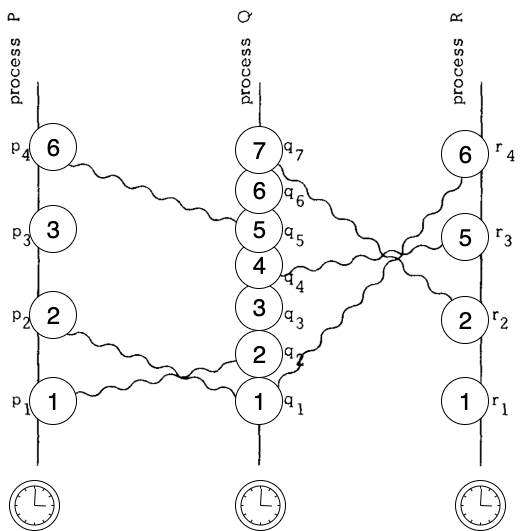
\includegraphics[width=\textwidth]{files/ClockDist-Logical-Clock.png}
		\end{figure}


	\end{column}
	\end{columns}


}

\frame
{
	\frametitle{Logical Clocks}

	\begin{columns}
	\begin{column}{0.6\textwidth}

		Implement the logical clock:

		\begin{itemize}
			\item<2-> Each process $P_i$ maintains $C_i$
			\item<3-> $P_i$ increments $C_i$ for each new events
			\item<4-> Each message $m$ is identified with the event $a$ that sends it, and timestamped by $T_m=C_i\langle a\rangle$
			\item<5-> On receiving message $m$, $P_j$ sets $C_j$ to be greater than both $T_m$ and current clock value
		\end{itemize}


	\end{column}
	\begin{column}{0.4\textwidth}

		\begin{figure}[ht!]
		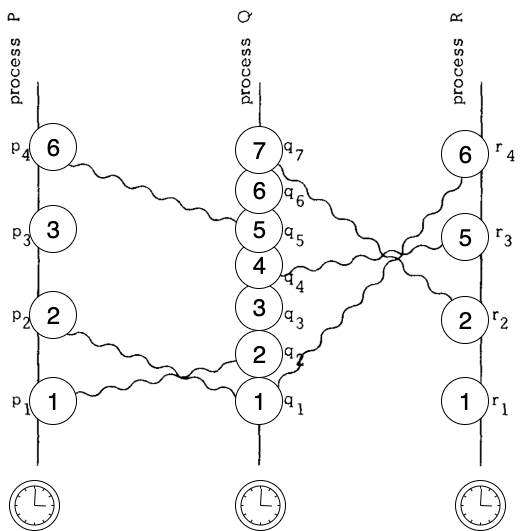
\includegraphics[width=\textwidth]{files/ClockDist-Logical-Clock.png}
		\end{figure}


	\end{column}
	\end{columns}


}

\frame
{
	\frametitle{Logical Clocks}

	\begin{columns}
	\begin{column}{0.6\textwidth}

		Example


	\end{column}
	\begin{column}{0.4\textwidth}

		\begin{figure}[ht!]
		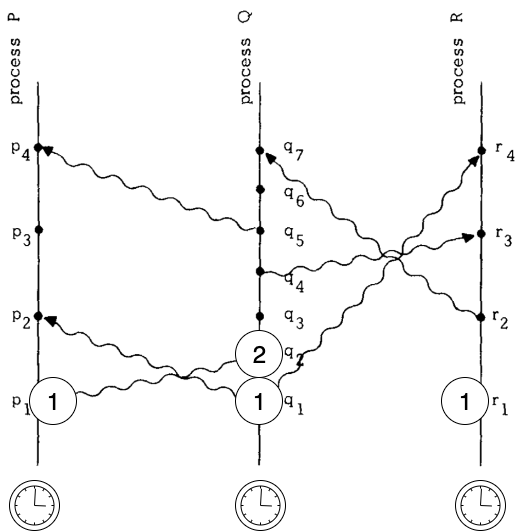
\includegraphics[width=\textwidth]{files/ClockDist-Impl-Logical-Clock-1.png}
		\end{figure}


	\end{column}
	\end{columns}
}

\frame
{
	\frametitle{Logical Clocks}

	\begin{columns}
	\begin{column}{0.6\textwidth}

		Process $Q$ receives message $p_1$, updates clock to $2$


	\end{column}
	\begin{column}{0.4\textwidth}

		\begin{figure}[ht!]
		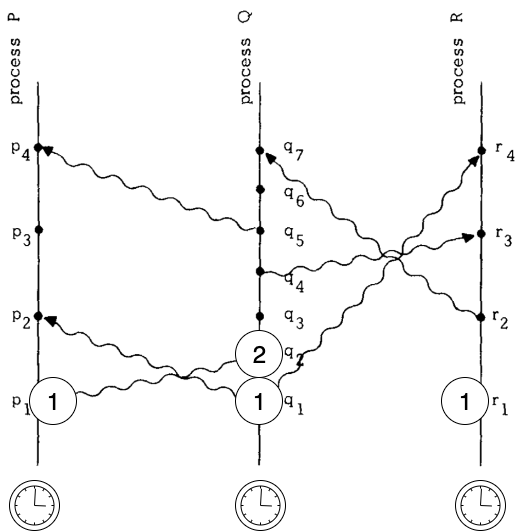
\includegraphics[width=\textwidth]{files/ClockDist-Impl-Logical-Clock-1.png}
		\end{figure}


	\end{column}
	\end{columns}


}

\frame
{
	\frametitle{Logical Clocks}

	\begin{columns}
	\begin{column}{0.6\textwidth}

		Process $P$ receives message $q_1$, updates clock to $2$


	\end{column}
	\begin{column}{0.4\textwidth}

		\begin{figure}[ht!]
		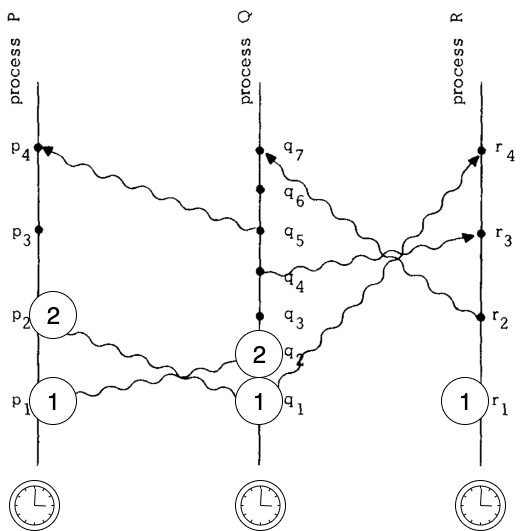
\includegraphics[width=\textwidth]{files/ClockDist-Impl-Logical-Clock-2.png}
		\end{figure}


	\end{column}
	\end{columns}


}

\frame
{
	\frametitle{Logical Clocks}

	\begin{columns}
	\begin{column}{0.6\textwidth}

		Proceeds until $Q$ sends a message to $R$ at event $q_4$ with timestamp 4


	\end{column}
	\begin{column}{0.4\textwidth}

		\begin{figure}[ht!]
		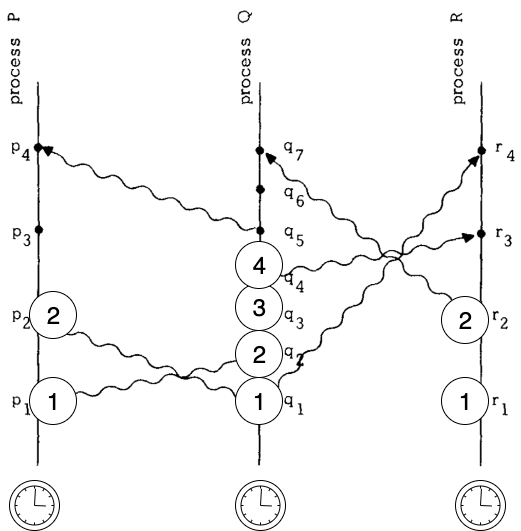
\includegraphics[width=\textwidth]{files/ClockDist-Impl-Logical-Clock-3.png}
		\end{figure}


	\end{column}
	\end{columns}


}

\frame
{
	\frametitle{Logical Clocks}

	\begin{columns}
	\begin{column}{0.6\textwidth}

		Process $R$ receives the message with timestamp 4, and updates clock to 5


	\end{column}
	\begin{column}{0.4\textwidth}

		\begin{figure}[ht!]
		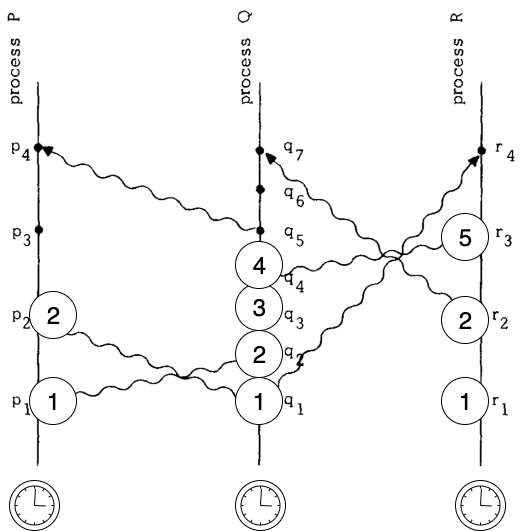
\includegraphics[width=\textwidth]{files/ClockDist-Impl-Logical-Clock-4.png}
		\end{figure}


	\end{column}
	\end{columns}


}

\frame
{
	\frametitle{Logical Clocks}

	\begin{columns}
	\begin{column}{0.6\textwidth}

		Process $Q$ sends message to $P$ with timestamp 5


	\end{column}
	\begin{column}{0.4\textwidth}

		\begin{figure}[ht!]
		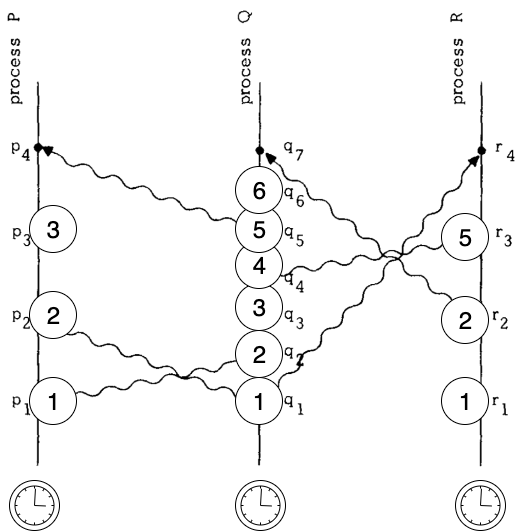
\includegraphics[width=\textwidth]{files/ClockDist-Impl-Logical-Clock-5.png}
		\end{figure}


	\end{column}
	\end{columns}


}

\frame
{
	\frametitle{Logical Clocks}

	\begin{columns}
	\begin{column}{0.6\textwidth}

		Process $P$ updates clock on receiving message with timestamp 5.
		Clocks of processes $Q$ and $R$ are not affected by messages.


	\end{column}
	\begin{column}{0.4\textwidth}

		\begin{figure}[ht!]
		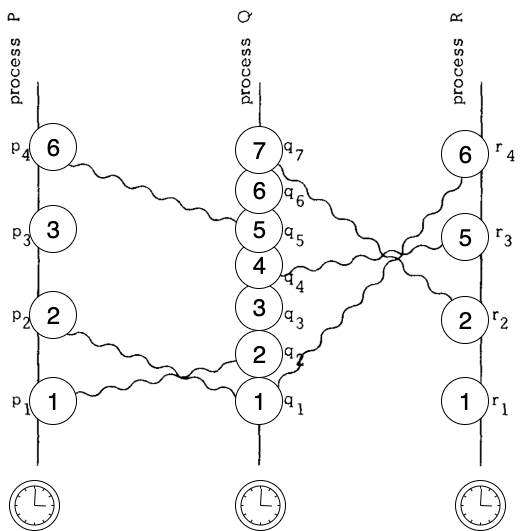
\includegraphics[width=\textwidth]{files/ClockDist-Impl-Logical-Clock-6.png}
		\end{figure}


	\end{column}
	\end{columns}


}

\frame
{
	\frametitle{Total Ordering}
	\begin{columns}
	\begin{column}{0.6\textwidth}


		With the logical clock, we are ready to define a total order ``$\Rightarrow$'' for all events.

		\begin{itemize}
			\item<2-> Use the logical clock as the primary index
			\item<3-> Define a total order $\prec$ over the processes as secondary index
			\item<4-> Formally, for events $a$ in $P_i$ and $b$ in $P_j$, $a\Rightarrow b$ if and only if either
				\begin{itemize}
					\item $C_i\langle a\rangle < C_j\langle b\rangle$ or;
					\item $C_i\langle a\rangle = C_j\langle b\rangle$ and $P_i\prec P_j$
				\end{itemize}
		\end{itemize}

	\end{column}
	\begin{column}{0.4\textwidth}

		\begin{figure}[ht!]
		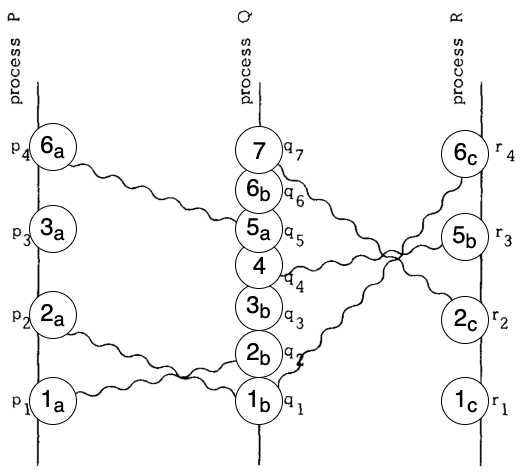
\includegraphics[width=\textwidth]{files/ClockDist-Total-Order.png}
		\end{figure}


	\end{column}
	\end{columns}
}

\section{Mutual Exclusion}
\frame
{
  \frametitle{Mutual Exclusion}
  Mutual exclusion is common in implementing resource sharing in distributed systems.
  In our protocol, we assume:
  \begin{itemize}
  	\item<2-> Fixed collection of processes
  	\item<3-> Single resource
  \end{itemize}
  \onslide<4-> We want a protocol satisfying following conditions:
  \begin{itemize}
  	\item<5-> \textbf{(I) Mutual exclusion}: once granted, must be released before granted again.
  	\item<6-> \textbf{(II) In Order}: Earlier requests granted ealier
  	\item<7-> \textbf{(III) Accessibility}: If every granted request eventually releases, then every request is eventually granted.
  \end{itemize}

  \onslide<1->\begin{figure}[ht!]
  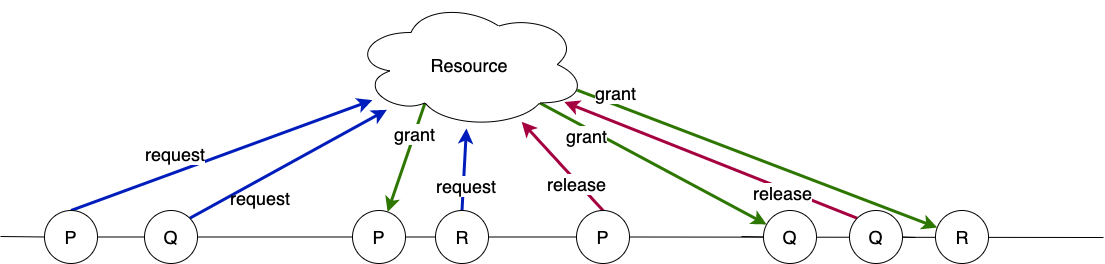
\includegraphics[width=0.8\textwidth]{files/ClockDist-Mutual-Exclusion.png}
  \end{figure}

}

\frame
{
  \frametitle{Mutual Exclusion}

  To simplify the implementation, some assumptions are needed to avoid extra details.
  \begin{itemize}
  	\item<2-> For any $P_i$ and $P_j$, the messages sent from $P_i$ to $P_j$ are received in order
  	\item<3-> Every message is eventually received
  	\item<4-> A process can send messages directly to every other process
  \end{itemize}


  %\onslide<5->\begin{block}{Remark}
  %\onslide<5-> Are they realizable?
%
  %\onslide<6-> Of course, that's just what TCP/IP gives you.
  %\end{block}
}

\frame
{
  \frametitle{Mutual Exclusion}

  \onslide<2->Each process maintains its own \emph{request queue}.

  \begin{itemize}
  	\item<3-> If $P_i$ wants the resource, it sends a message $m=\langle T_m:P_i\text{ \emph{requests resource}}\rangle$ to every other process, and puts $m$ on its request queue
  	\item<4-> When $P_j$ receives $m$, it puts $m$ on its request queue, and sends an acknowledgement message to $P_i$
  \end{itemize}
  \onslide<1->\begin{figure}[ht!]
  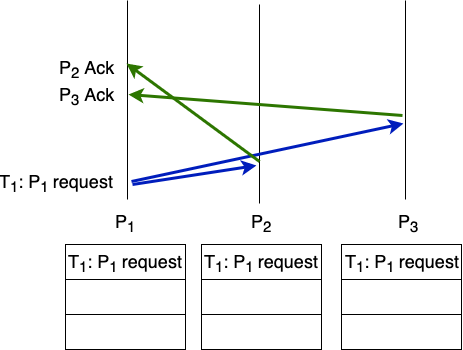
\includegraphics[width=0.5\textwidth]{files/ClockDist-Request.png}
  \end{figure}

}

\frame
{
  \frametitle{Mutual Exclusion}

  Releasing the resource works in similar way, without acknowledgement.

  \begin{itemize}
  	\item<2-> If $P_i$ wants to release the resource, it sends a message $\langle T_m':P_i\text{ \emph{releases resource}}\rangle$ to other processes, and removes any $\langle T_m:P_i\text{ \emph{requests resource}}\rangle$ from its request queue
  	\item<3-> When $P_j$ receives $\langle T_m':P_i\text{ \emph{releases resource}}\rangle$, it removes any $\langle T_m:P_i\text{ \emph{requests resource}}\rangle$ from its request queue
  \end{itemize}
  \begin{figure}[ht!]
  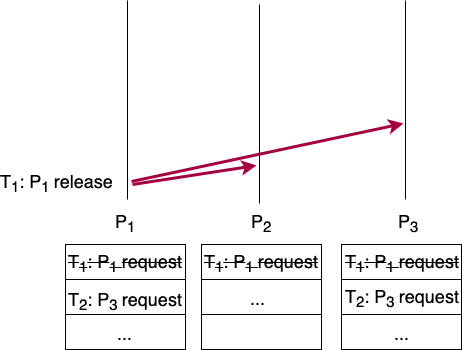
\includegraphics[width=0.5\textwidth]{files/ClockDist-Release.png}
  \end{figure}
}

\frame
{
  \frametitle{Mutual Exclusion}

  $P_i$ is granted the resource if the following conditions hold.

  \begin{itemize}
  	\item<2-> There is a $\langle T_m:P_i\text{ \emph{requests resource}}\rangle$ in its request queue ordered before any other messages inside the queue by relation ``$\Rightarrow$''
  	\item<3-> $P_i$ received the acknowledgements from every other process
  \end{itemize}
  \onslide<4-> Now $P_i$ can safely access the resource, assured that nobody else is granted the resource.

  \onslide<5-> But why does this work?
}

\frame
{
  \frametitle{Mutual Exclusion}
  The above protocol satisfies conditions (I)(II) and (III).

  \begin{itemize}
  	\item<2-> \textbf{Conditions I and II:} From the point of view of $m=\langle T_m:P_i\text{ \emph{requests resource}}\rangle$, any request $m'$ issued later by $P_j$ is in either of the following cases:
  		\begin{itemize}
  			\item Acknowledged by $P_i$, then $P_j$ must also have received $m$, and $m'$ is superceded by $m$ in $P_j$'s queue
  			\item Not acknowledged by $P_i$
  		\end{itemize}
  	In any case, $m'$ is not granted.
  	\onslide<3-> In summary, for any request $m$, no request issued later than $m$ will be granted before $m$ is released.
		\item<4-> \textbf{Condition III:} For each message $m=\langle T_m:P_i\text{ \emph{requests resource}}\rangle$:
			\begin{itemize}
				\item $m$ will be the oldest in $P_i$'s queue eventually
				\item $P_i$ will receive all acknowledgements eventually
			\end{itemize}
  \end{itemize}
}

\frame
{
  \frametitle{Mutual Exclusion}
  \begin{block}{Remark}
	  \begin{itemize}
	  	\item<2-> No centralized authority, everything happens automatically in sending and receiving messages
	  	\item<3-> Requires all parties trusted. Malicious party can easily forge timestamps, refuse to send acknowledgement, etc.
	  	\item<4-> The shared resource is an abstract concept, which can be anything
	  	\item<5-> Can be easily extended to multiple resources
	  \end{itemize}
	  \onslide<6-> Applied to consensus protocol?
	  \begin{itemize}
	  	\item<7-> Cryptographic mechanisms for trustlessness?
	  	\item<8-> Shared resource can be: leadership, write permission, ...
	  \end{itemize}
  \end{block}
}

\section{Physical Clock}
\frame
{
  \frametitle{Physical Clock}
  \onslide<+-> Let $t$ denote the real, ideal physical time, which is not available to any processes
  \begin{itemize}
  	\item<+-> $P_i$ only has access to a function of $t$, called a clock, denoted by $C_i(t)$ which is a (almost) differentiable function
  	\item<+-> The clock rates $dC_i(t)/dt$ approximate $1$
  	\item<+-> The idea is processes sending to each other synchronization messages, to ensure that $|C_i(t)-C_j(t)| \leq \varepsilon$ for all $t$ and all pairs of $i,j$, where $\varepsilon$ is related to parameters including:
  	\begin{itemize}
  		\item<+-> Global bound on message delay
  		\item<+-> Frequencies of synchronization messages sent to each other
  		\item<+-> Accuracy of the local clocks
  	\end{itemize}
  \end{itemize}
}

\frame
{
  \frametitle{Physical Clock}
	\begin{columns}
	\begin{column}{0.6\textwidth}
		The clocks run at different rates and start deviating from each other
	\end{column}
	\begin{column}{0.4\textwidth}

		\begin{figure}[ht!]
		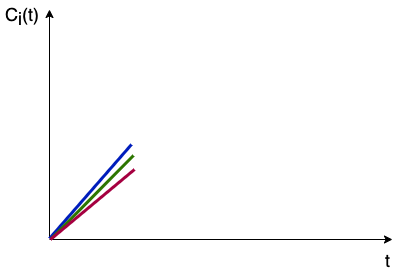
\includegraphics[width=\textwidth]{files/ClockDist-Physical-Clock-1.png}
		\end{figure}

	\end{column}
	\end{columns}
}

\frame
{
  \frametitle{Physical Clock}
	\begin{columns}
	\begin{column}{0.6\textwidth}
		The third process receives a message from second process, and resets clock.
	\end{column}
	\begin{column}{0.4\textwidth}

		\begin{figure}[ht!]
		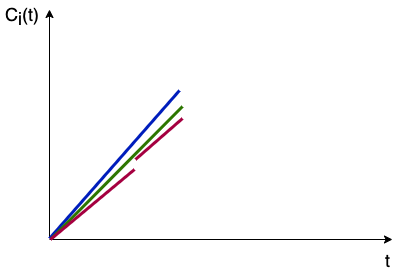
\includegraphics[width=\textwidth]{files/ClockDist-Physical-Clock-2.png}
		\end{figure}

	\end{column}
	\end{columns}
}

\frame
{
  \frametitle{Physical Clock}
	\begin{columns}
	\begin{column}{0.6\textwidth}
		The second process receives a message from first process, and resets clock.
	\end{column}
	\begin{column}{0.4\textwidth}

		\begin{figure}[ht!]
		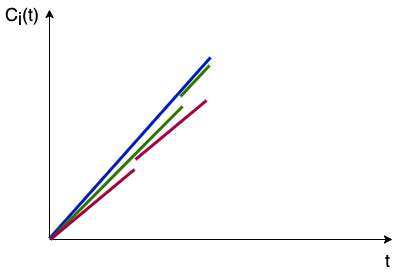
\includegraphics[width=\textwidth]{files/ClockDist-Physical-Clock-3.png}
		\end{figure}

	\end{column}
	\end{columns}
}

\frame
{
  \frametitle{Physical Clock}
	\begin{columns}
	\begin{column}{0.6\textwidth}
		The third process receives a message from first process, and resets clock.
	\end{column}
	\begin{column}{0.4\textwidth}

		\begin{figure}[ht!]
		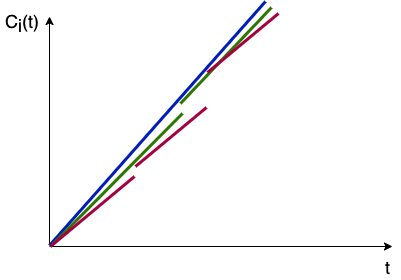
\includegraphics[width=\textwidth]{files/ClockDist-Physical-Clock-4.png}
		\end{figure}

	\end{column}
	\end{columns}
}

\frame
{
  \frametitle{Physical Clock}
	\begin{columns}
	\begin{column}{0.6\textwidth}
		Given appropriate assumptions, the clocks are syncronized within bounded error.
	\end{column}
	\begin{column}{0.4\textwidth}

		\begin{figure}[ht!]
		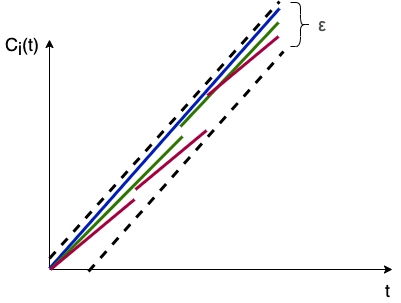
\includegraphics[width=\textwidth]{files/ClockDist-Physical-Clock-5.png}
		\end{figure}

	\end{column}
	\end{columns}
}

\frame
{
  \frametitle{Summary}
  \begin{itemize}
  	\item Total ordering
  		\begin{itemize}
  			\item Partial order ``happens before'' on events: $\to$
  			\item Logical clock that respects ``$\to$''
  			\item Logical clock + Total order on processes $\Rightarrow$ total order on events
  		\end{itemize}
  	\item Protocol that achieves mutual exclusion, and something more
  	\item Physical clock
  \end{itemize}
}

\iffalse
\section{Physical Clock}
\frame
{
  \frametitle{Physical Clock}
  Let $t$ denote the physical time, and $C_i(t)$ be the value of clock $C_i$.

  \begin{itemize}
  	\item\pause $C_i(t)$ is continuous and differentiable function of $t$ except for jump discontinuities
  	\item\pause $dC_i(t)/dt$ is the rate of the clock at $t$, assumed that $\left|dC_i(t)/dt-1\right|<\kappa\ll 1$
  \end{itemize}

  \pause
  \begin{figure}[ht!]
  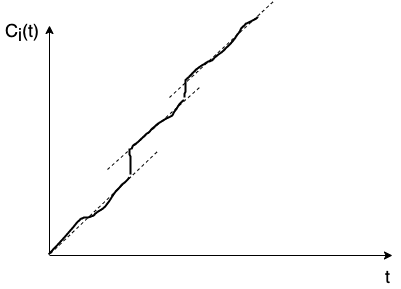
\includegraphics[width=0.4\textwidth]{files/ClockDist-Physical-Clock.png}
  \end{figure}

}

\frame
{
  \frametitle{Physical Clock}
  We need a protocol to make sure that all the $C_i(t)$'s are synced, i.e. for all $i,j$:

  \[|C_i(t)-C_j(t)|<\varepsilon\]

  \pause
  We need some assumptions and notations before describing the protocol.

  \begin{itemize}
  	\item\pause If a message $m$ is sent at time $t$, received at time $t'$, the total delay is $\nu_m=t'-t$, which is not known to the receiver
  	\item\pause We assume that the receiving process knows some minimum delay $\mu_m\leq\nu_m$
  	\item\pause Denote by $\xi_m=\nu_m-\mu_m$ the \emph{unpredictable delay}
  \end{itemize}
}

\frame
{
  \frametitle{Physical Clock}
  The protocol executes as follows.

  \begin{itemize}
  	\item<2-> If $P_i$ does not receive message at time $t$, then $P_i$ does not modify $C_i$, and $dC_i(t)/dt\approx 1$
  	\item<3-> When $P_i$ sends a message $m$, it appends timestamp $T_m=C_i(t)$ in the message
  	\item<4-> If at time $t'$, $P_i$ receives a message $m$ with timestamp $T_m$, $P_i$ resets $C_i(t')$ to $\max(C_i(t'), T_m+\mu_m)$
  \end{itemize}
}

\frame
{
  \frametitle{Physical Clock}
  \begin{block}{Theorem}
  Assume a strongly connected graph of processes with diameter $d$ follows the above protocol. Assume that for any message $m$, $\mu_m\leq\mu$ for some constant $\mu$, and that for all $t\geq t_0$:
  \begin{enumerate}
  	\item $|dC_i(t)/dt-1|\leq\kappa\ll 1$
  	\item every $\tau$ seconds a message $m$ with $\xi_m<\xi$ is sent over every arc, where $\tau$ and $\xi$ are constants
  \end{enumerate}
  Then for all $i,j$: $|C_i(t)-C_j(t)|<\varepsilon$ where $\varepsilon\approx d(2\kappa\tau+\xi)$ for all $t\gtrsim t_0+\tau d$ and $\mu+\xi\ll\tau$
  \end{block}
}

\frame
{
  \frametitle{Physical Clock}
  \begin{block}{Proof Sketch}
  \begin{enumerate}
  	\item<2-> Prove that for any $i,j$ and any $t,t_1$ with $t_1\geq t_0$ and $t\geq t_1+d(\tau+\nu)$:
  	\[C_i(t)\geq C_j(t_1)+(1-\kappa)(t-t_1)-d\xi\]
  	\item<3-> Prove that for any $t,t_x$ with $t\geq t_x\geq t_0+\mu/(1-\kappa)$ there is a process $P_q$ and a time $t_1$ with $t_x-\mu/(1-\kappa)\leq t_1\leq t_x$ such that for all $i$:
  	\[C_i(t)\leq C_q(t_1)+(1+\kappa)(t-t_1)\]
  	\item<4-> Prove that for all $i,j$:
  	\[|C_i(t)-C_j(t)|\lesssim d(2\kappa\tau+\xi)\]
  	for all $t\gtrsim t_0+d\tau$
  \end{enumerate}
  \end{block}
}

\frame
{
  \frametitle{Physical Clock}
  \begin{block}{Step 1}
  \begin{enumerate}
  	\item<1-> Define $C_i^t$ to be a clock set equal to $C_i$ at time $t$ and runs at the same rate as $C_i$, but is never reset. Then we have for any $t'\geq t$, $C_i^t(t')\leq C_i(t')$
  	\item<2-> Suppose $P_1$ at time $t_1$ sends a message to $P_2$ which is received at $t_2$, then for any $t\geq t_2$
  	\[C_2^{t_2}(t)\geq C_1(t_1)+(1-\kappa)(t-t_1)-\xi\]
  	\item<3-> For any $P$ and $P'$, there is a sequence $P=P_0,P_1,\cdots,P_{n+1}=P'$, $n\leq d$, for each pair of $P_i,P_{i+1}$, assume $P_i$ receives a message at $t_i$, sends a message to $P_{i+1}$ at $t_i'$, and $P_{i+1}$ receives message at $t_{i+1}$, we can find $t_i'-t_i\leq\tau$, $t_{i+1}-t_i'\leq\nu$. Then we have
  	\[C_{n+1}(t)\geq C_{n+1}^{t_{n+1}}(t) \geq C_1(t_1)+(1-\kappa)(t-t_1)-n\xi\]
  \end{enumerate}
  \end{block}
}

\frame
{
  \frametitle{Physical Clock}
  \begin{block}{Step 2}
  \begin{enumerate}
  	\item<1-> Assign a clock $C_m$ to each message $m$ sent at $t$ and received at $t'$, with $C_m(t)=t$ and constant rate $dC_m/dt=\mu_m/(t'-t)$
  	\item<2-> For any time $t_x\geq t_0+\mu/(1-\kappa)$, let $C_x$ be the clock with largest value at $t_x$. Consider two cases:
  		\begin{enumerate}
  			\item<3-> $C_x$ is $C_q$ for some process $P_q$, then for any $i$ and $t\geq t_x$
  			\[C_i(t)\leq C_q(t_x)+(1+\kappa)(t-t_x)\]
  			\item<4-> $C_x$ is $C_m$ for some message $m$ sent at $t_1$ by process $P_q$, then $t_x\leq t_1+\mu/(1-\kappa)$, and for any $i$ and $t\geq t_1$
  			\[C_i(t)\leq C_q(t_1)+(1+\kappa)(t-t_1)\]
  		\end{enumerate}
  	\item<5-> Let $t_1=t_x$ in first case, then we have $t_1$ such that $t_x-\mu/(1-\kappa)\leq t_1\leq t_x$, and there exists process $P_q$ such that for all $t\geq t_x$ and for all $i$ the above equation holds.
  \end{enumerate}
  \end{block}
}

\frame
{
  \frametitle{Physical Clock}
  \begin{block}{Step 3}
  \begin{enumerate}
  	\item<1-> Now we conclude that there always exists process $P_q$ and time $t_1$ such that
  	\[C_q(t_1)+(1-\kappa)(t-t_1)-d\xi\leq C_i(t)\leq C_q(t_1)+(1+\kappa)(t-t_1)\]
  	\item<2-> Let $t=t_x+d(\tau+\nu)$, update the above bounds
  	\begin{eqnarray*}C_q(t_1)+(t-t_1)-\kappa d(\tau+\nu)-d\xi\leq C_i(t)\\\leq C_q(t_1)+(t-t_1)+\kappa[d(\tau+\nu)+\mu/(1-\kappa)]\end{eqnarray*}
  	\item<3-> By $\mu\leq\nu\ll\tau$ and $\kappa\ll 1$, and the fact that the above holds for all $i$
  	\[|C_i(t)-C_j(t)|\lesssim d(2\kappa\tau+\xi)\]
  \end{enumerate}
  \end{block}
}
\fi

\frame
{
  \center\huge{Q\&A}
}

\end{document}
